%\pagebreak
\chapter{Meta-Modeling Evaluation}
\label{ch:eval}

%\markboth{EDD Usability}{}

This chapter discusses the use of Embodied-Driven Design (EDD) meta-models to address body limitations in five different projects. Each of these projects highlights a specific scenario which EDD meta-modeling resolves. The four meta-modeling approaches described here are: 
\begin{itemize}
    \item Direct Body Transfer: Modalities are directly mapped from the body to the representation, used for functional body modalities (no alteration is required).

    \item Representation alteration: Different type of representation is used to overcome a physical limitation of the body.
    
    %meta-model to overcome physical limitations by using hybrid virtual/physical representation.
    \item Topology Reconfiguration: Change the association and mapping of the modalities between the body and representation to overcome a physical disability, or to alter modality's function.

    %meta-model to manipulate the internal body schema by remapping the number of body limbs.
    \item Modality Expansion: Augment a sensory modality by using different sources of feedback from multiple representations, or expand modality's operation to multiple modalities simultaneously.

    %meta-model to expand perceptual modalities to multiple locations.
\end{itemize}

These four approaches are illustrated in \Figure{fig:eval-overview-MetaModelReq} along the association with the five projects discussed here. Each of these projects uses one or more meta-modeling approach to resolve body related criteria. Design considerations and implementation of these projects using EDD, along the conducted observations and results are detailed here.

\begin{figure}[h!]
  \centering
	  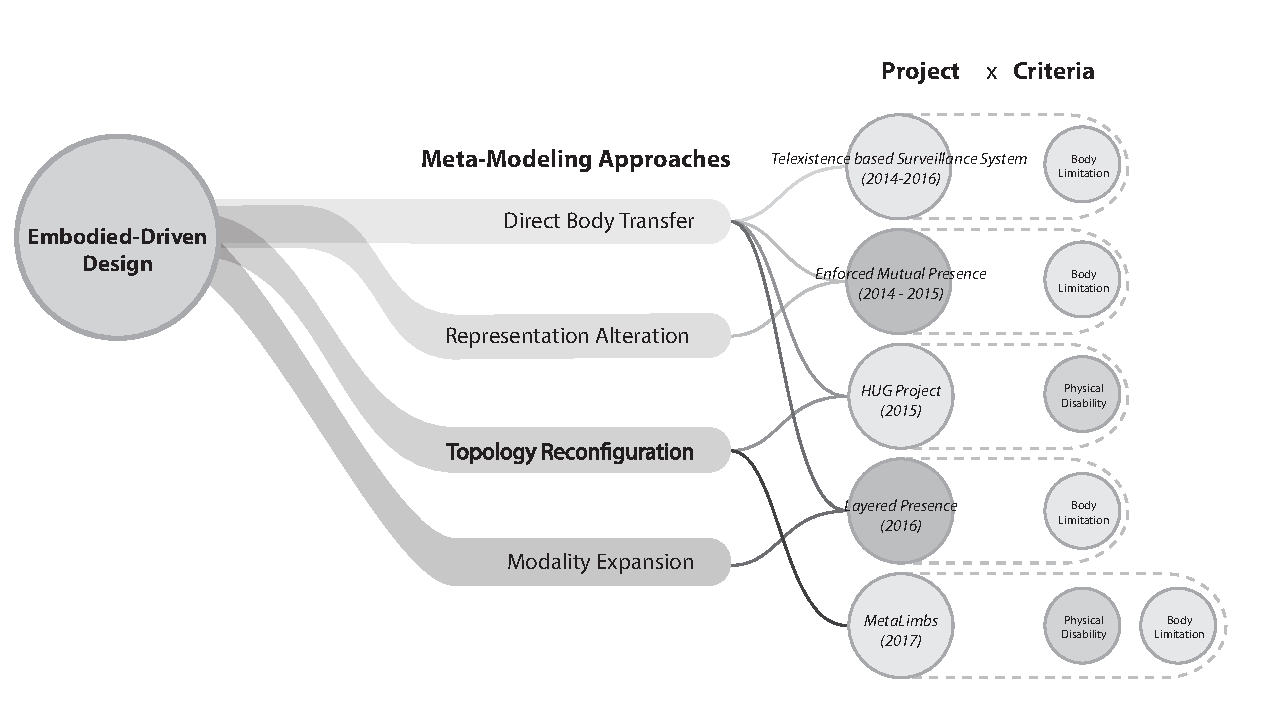
\includegraphics[width=1\linewidth]{figures/intro/MetaModelingOverview.pdf}
  \captionsetup{justification=centering}
  \caption{An overview of the four meta-models along the five projects discussed in this chapter.}
  \label{fig:eval-overview-MetaModelReq}
\end{figure}


%%%%%%%%%%%%%%%%%%%%%%%%%%%%%%%%%%%%%%%%%%%%%%%%%%%%%%%%%%%%%%%%%%%%%%%%%%%%%%%%%%%%%%%%%%

%\pagebreak
\section{Telexistence based Surveillance System}
\label{sec:eval-txSys}
%NEDO-Obayashi


\begin{comment}

\begin{figure}[h!]
  \centering
	  \includegraphics[width=1\linewidth]{figures/eval/MetaModels/Tx-Meta.pdf}
  \captionsetup{justification=centering}
  \caption{Use of MetaModeling approach to address Telexistence based Surveillance System (body limitations).}
  \label{fig:eval-nedo-MetaModelReq}
\end{figure}

\end{comment}

Teleoperation, in general, has begun as a mean enabling human to operate a sub-system from a remote and a safe place. The disasters that occurred during the course of the past 50 years (mainly nuclear and hazardous disasters) has sparked the need to build safe systems which experts can use and access the hazardous regions for maintenance or collect data and samples regarding the reason of the fault. Most recently, Fukushima Daiichi nuclear disaster in 2011 has resulted to launch several government-funded research programs to avoid similar cases in the future, and to build systems which the current teleoperated and AI-based systems failed to provide adequate access to the reactor. One of the most important requirements for such systems was the quick deployment to the scene to collect early information, and to allow expert people not used for teleoperation to quickly manage these systems with a minimum amount of training.



\begin{figure}[t!]
  \centering
	  \includegraphics[width=1\linewidth]{figures/eval/NEDO/Overview.pdf}
  \captionsetup{justification=centering}
  \caption{An overview of Telexistence based surveillance system.}
  \label{fig:usability-nedo-overview}
\end{figure}


This project was established to address the previous requirements and need through a remotely operated navigation systems that can be deployed in the damaged location which human can not access. A collaboration between Keio University and Obayashi corporation started in September 2014 and continued until the end of 2016, funded by New Energy and Industrial Technology Development Organization (NEDO). During this collaboration, we developed an unmanned survey robot that enables remote investigation of the collapsed site. An overview of the developed system is shown in \Figure{fig:usability-nedo-overview}. The system mainly consists of a remotely operated vehicle through a telexistence based system located in the driver seat of the crawler, a penetration rod used to collect samples from the ground, a stable and long range wireless network access points and repeaters, and an operation cockpit which contains the tracking and control tools of the vehicle and robot, and the perceptual devices to deliver feedback from the representation. Each of these sub systems was handled separately by different corporations and research facilities. An overview of the general specifications for this system is listed in \Table{table:nedo-specs}. Our main contribution in this project is the development and deployment the operation cockpit as well as the telexistence system used in the crawler.



\begin{table}[t!]
\begin{tabular}{|
>{\columncolor[HTML]{EFEFEF}}l |l|}
\hline
\textbf{Specification}    & \cellcolor[HTML]{EFEFEF}\textbf{Details}                                                          \\ \hline
Vehicle Dimensions        & 4340mm x 1740mm x 1650mm                                                                          \\ \hline
Vehicle Net Weight        & 1900kg                                                                                            \\ \hline
Image Acquisition         & \begin{tabular}[c]{@{}l@{}}Stereo camera system \\ + rear omni directional camera\end{tabular}    \\ \hline
Vehicle Driving Mechanism & Operator hand held controller                                                                     \\ \hline
Visual Presentation       & \begin{tabular}[c]{@{}l@{}}Head Mounted Display \\ + screens for external monitoring\end{tabular} \\ \hline
Stereo Visuals Resolution & 480p@60FPS - 720p@60FPS                                                                           \\ \hline
Operation Mechanism       & Head motion (position + rotation)                                                                 \\ \hline
Visual/Operation Latency  & Less than 150ms                                                                                   \\ \hline
Wireless Communication    & 2.4 GHz wireless LAN                                                                              \\ \hline
Communication Distance    & Up to 2 km (with a wireless repeater)                                                             \\ \hline
\end{tabular}
\centering
\caption{General specifications for the surveillance system.}
\label{table:nedo-specs}
\end{table}


\subsection{Design of Remotely Operated Representation}

For the development of the telexistence robot, the challenge was to maintain high degree of operation of the robot in terms of both performance time and quality of operation in the remote location. Vehicle driving was a part of the tasks to be operated, thus 3DOF telexistence robot is not sufficient since parallax motion is required when driving. To achieve such requirement, a custom made 6DOF telexistence system was developed (mechanical design by KAWABUCHI Mechanical Engineering Laboratory, Inc.) as shown in \Figure{fig:usability-nedo-torso}. The robot operation system follows the same protocol for communication and control as the one designed for the toolkit (described in \Chapter{ch:impl}), thus the visual, auditory, and body control modalities are compatible with EDD framework requirements. 


\begin{figure}[h!]
  \centering
	  \includegraphics[width=1\linewidth]{figures/eval/NEDO/TORSO2.pdf}
  \captionsetup{justification=centering}
  \caption{6DOF Telexistence system (TORSO).}
  \label{fig:usability-nedo-torso}
\end{figure}



The system development and testing took several iterations and run-tests to evaluate the degree of control of the robot. Initial experiments to operate the vehicle is shown in \Figure{fig:usability-nedo-exp1}. The operator vision is mapped to the robot visual feedback, and his head motion controls the representation movement. The modality data flow is managed by EDD framework. The evaluation layout for the test field of the initial experiments is shown in \Figure{fig:usability-nedo-exp-setup}, and located at Obayashi corporation machinery factory in Kawagoe City. The operator had to navigate through set of land marks (cones) without touching them while driving. The vehicle used was a backhoe that has a dedicated remote control panel.

\begin{figure}[htpb]
  \centering
	  \includegraphics[width=1\linewidth]{figures/eval/NEDO/Expermint1.pdf}
  \captionsetup{justification=centering}
  \caption{An initial set of experiments of using remote operation.}
  \label{fig:usability-nedo-exp1}
\end{figure}

Total of 40 users operated the system, 35 out of them had no previous experience at driving the backhoe. Before operation, the users would be taught how navigate the vehicle using the remote controller. Afterwards, the pilots would access the remote robot via HMD and drive through the field. As a result of the tests, we found that the pilots were capable to maneuvering precisely through the landmarks since they had a correspondence mapping between the visual modality and the robot stereo cameras, thus the depth perception was correctly matched. Also, the low latency transmission played an important role at reducing the visual sickness of operation, and at precise decision making when making turns. Pilots even used to see through the mirrors located inside the backhoe to have wider awareness of the location, cones, and walls nearby, just as if they were in the driving seat. 

\begin{figure}[htpb]
  \centering
	  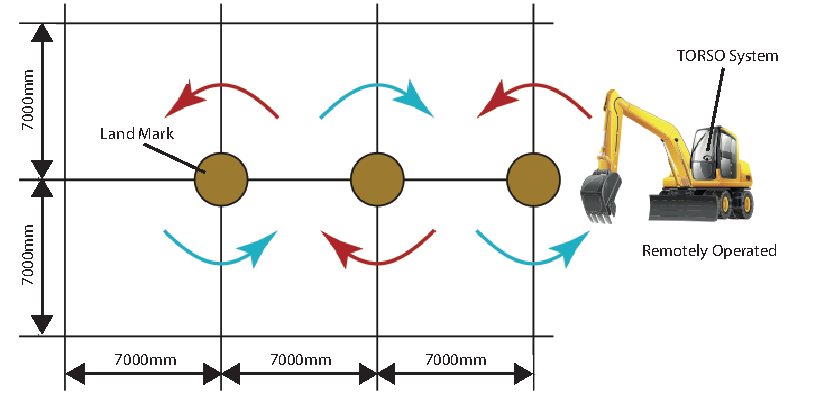
\includegraphics[width=1\linewidth]{figures/eval/NEDO/experiment.pdf}
  \captionsetup{justification=centering}
  \caption{Remote navigation using TORSO system.}
  \label{fig:usability-nedo-exp-setup}
\end{figure}

The next stage of the project was carried to deploy the robot into the crawler vehicle. The vehicle operation differs from backhoe operation in terms of scale and operations that should be conducted using it. The vehicle was designed to operate in terrain environment, and under various weather conditions (rainy, windy, ... etc). The finalized system after being integrated with the vehicle is shown in \Figure{fig:usability-nedo-exp2}. The operator is provided with two types of operation: using the HMD for driving and inspection, and external screen connected to an omni-directional camera mounted on the top of the vehicle to gain a global view of the vehicle and the inspection equipment.

\begin{figure}[htpb]
  \centering
	  \includegraphics[width=1\linewidth]{figures/eval/NEDO/Expermint2.pdf}
  \captionsetup{justification=centering}
  \caption{Second phase of remotely operated driving system.}
  \label{fig:usability-nedo-exp2}
\end{figure}

\begin{figure}[b!]
  \centering
	  \includegraphics[width=1\linewidth]{figures/eval/NEDO/simulator.pdf}
  \captionsetup{justification=centering}
  \caption{Virtual navigation and operation platform.}
  \label{fig:usability-nedo-simulator}
\end{figure}

To support the operation in large-scale environments, a virtual navigation system was developed \Figure{fig:usability-nedo-simulator} that uses the concepts of virtual presence to replicate the same experience of driving the actual vehicle, and which communicate in real-time with the physical system. Various point of views can be used in the virtual environment which would provide a higher degree of flexibility in navigation. A photogrammetry based model of the actual location is generated offline (developed by a third-party) and rendered in the virtual space. The vehicle coordinates are captured via a GNSS module (u-blox Neo 7) embedded into the vehicle and mapped into the coordinates of the virtual environment. This transitional environment between the first point of view (robot side), the third person of view (simulator side), and bird point of view (simulator side) would expand the spatial awareness of the operator beyond what traditional teleoperated systems can provide. %The final evaluations of the system took place at Unzen in Nagasaki prefecture.


\subsection{Telexistence System Meta-Modeling}

In this project, direct body transfer meta-modeling approach were used to map operator's body with the used representation. \Figure{fig:eval-EDD-NEDO} shows the target meta-model and body mapping between the user and the robot. Since the system is intended to be operated same as being physically in the vehicle, and by operators without physical disabilities, the modality mapping is direct. The head modality contains spatial information of user's head (position and rotation), which is mapped to TORSO robot. The robot maintains same coordinates with the user, and in return provides the visual (stereo images) and auditory (bin-aural) information. Such mapping directly matches the operator with the robot. 

\begin{figure}[htpb]
  \centering
  \includegraphics[width=0.95\linewidth]{figures/eval/EDD/EDD-NEDO.pdf}
  \captionsetup{justification=centering}
  \caption{An overview of the target meta-model for Telexistence type systems.}
  \label{fig:eval-EDD-NEDO}
\end{figure}

The actual meta-model developed is shown in \Figure{fig:usability-nedo-metamodel}. The meta-model contains two types of blocks: Body blocks (HMD Node, Body, Microphone, and User Node), and representation blocks (Robot and Simulated). For this particular design, no transfer blocks were used.


\begin{figure}[htpb]
  \centering
  \captionsetup{justification=centering}
  \includegraphics[width=1\linewidth]{figures/eval/NEDO/ObayashiEDD.png}
  \caption{A screen-shot of EDD Meta-modeling editor describing the association user's between body and two representations: physical and simulated.}
  \label{fig:usability-nedo-metamodel}
\end{figure}



\subsection{Discussion}


This project was an evidence that the presence of certain modalities (postural, vision) in the representation is sufficient to mediate body state in a bi-directional manner. In scenarios which the operation of the system is required to be immediate without any body reconfiguration or change in operation, direct body transfer can be used. This maintains the quality of embodied use of the representation. Compared with telepresence type of systems, the subjective evaluation it showed that the use of such body mapping with a representation has enhanced the quality of navigation and spatial understanding at the remote sites.

The digitization of body and operation and the use of mediated representation can also leverage the possibilities of what a body can perform, can sense, and can operate. For example, when the simulator environment was deployed, sensory data from drones were possible to integrate within the same proxy the operator used in his operation of the robot. Initial tests were also conducted to integrate Enforced Presence into the operation so the operator could see his hands and controller. The operators did report they had better awareness and less motion and visual sickness, however in later stages of the project, virtual hands were removed due to some design constraints of the cockpit.

 %Nonetheless, due to some imperfect matching of the slave system specifications such as the latency (an average of $148ms \pm27$) and drop of the framerate due to the variant quality of connectivity (bandwidth drops, wireless signal occlusion). 

%%%%%%%%%%%%%%%%%%%%%%%%%%%%%%%%%%%%%%%%%%%%%%%%%%%%%%%%%%%%%%%%%%%%%%%%%%%%%%%%%%%%%%%%%%

%\pagebreak
\section{Enforced Mutual Presence} 
\label{sec:eval-enforced}

\begin{comment}
\begin{figure}[htpb]
  \centering
	  \includegraphics[width=1\linewidth]{figures/eval/MetaModels/ET-Meta.pdf}
  \captionsetup{justification=centering}
  \caption{Use of MetaModeling approach to address Enforced Mutual Presence (body limitations).}
  \label{fig:eval-ET-MetaModelReq}
\end{figure}
\end{comment}

Enforced Mutual Presence uses representation alteration blocks to compensate non available physical representation using a virtual one. This use-case leverage the current telepresence systems which lacks the physical attributes of presenting human body, in which the user fails to observe his body being immersed in the teleoperated robot side. Also, as an extension of this work, a mutual body presentation is used to compensate the remote body representation, so the remote participants would be aware of the state of user's body and his actions. Enforced Mutual Presence addresses the following points:
\begin{itemize}
\item User’s body representation in a physical environment.
\item Preserving body ownership during teleoperation.
\item Presenting user’s body visuals to remote observers.
\end{itemize}




Three design aspects \cite{biocca1997cyborg,bracken2010immersed} contributes in achieving mutual presence and the awareness of being presented in a specific environment: spatial presence, self presence, and social presence. Spatial presence is to be capable to interact with the environment. Self presence can be described as to be able to observe our bodies being presented in the environment, and aware of its posture at any given moment. The social presence is how we observe social interaction with other people within one environment. 

To address the first key point ``spatial presence'' the user should have direct access to the environment as if he is located there, with the freedom to move and navigate via an alternative representation of his body. The user should be able to move freely and independently his head and body, and according to that, the slave robot should follow and update user’s visuals of the remote place. We avoid using any physical or tangible controller (such as a joystick or keyboard) to control motion and rotation speed of the slave robot. This is important because if the user is aware of the presence of a physical controller, then the coherence between the local and remote place will break. So an intuitive and natural interface is required to maintain spatial coherence. Body as a joystick concept was used to drive the robot spatial motion in the remote place. The concept uses body motion (leaning forward,backward, and sideways) to control the motion vector of the robot. This motion correlation helps to maintain the same motion/optical flow between the body and the visuals observed remotely.

The second point ``self presence'' is the fact the user should have physical awareness of his body’s presence. The user validates his existence in a specific place by observing his body’s visuals as he expects, maintaining the ownership relation with his body. In this work, we found that observing body visuals is an effective factor to maintain the seamless sense of presence for the user, so image-based method is developed which captures egocentric images of user’s body visuals, and superimpose it into the remote place. 

The final point addressed is ``social presence''. In order for the user to communicate effectively with other people in a different location, mutual communication between both sides should be maintained. As in  ``spatial presence'' the user is aware of the surroundings and people around, those people should be capable to understand what the user wants in return. It is commonly to user an LCD panel only to show user’s body, however this method is not capable to provide spatial interaction in the 3D space. As an alternative, we propose to project user’s body visuals in robot side, so the user can visually affect in the remote place, allowing remote observers to visualize his body.

\begin{figure}[t!] 
\centering
  \captionsetup{justification=centering}
\includegraphics[width=1\textwidth]{figures/eval/ET/ET.pdf}
\caption{Enforced Mutual Presence overview (A) the first person view for the user showing superimposed virtual hands, (B) user's hands are projected externally so others can mutually see, and (C) virtual hands are projected on an arbitrary surface.}
  \label{fig:eval-ET}
\end{figure}

\Figure{fig:eval-ET} shows a physical telexistence system combined with projected body visuals of the operating user. \Figure{fig:eval-ET} (A) shows what the user sees in the remote place while using his hands. The body visuals are preserved and projected back into his field of view in a natural and correspondent manner to his actual body. While \Figure{fig:eval-ET} (B) \& (C) shows what the remote participants observe: an extension of operator's body visual projected into the remote surfaces making it easy to understand what the user is pointing at. This design helps to overcome body physical limitations of the representation as well as increase sense of bodily presence. 



\begin{figure}[htpb]
  \centering
  \includegraphics[width=0.95\linewidth]{figures/eval/EDD/EDD-Mutual.pdf}
  \captionsetup{justification=centering}
  \caption{An overview of the target meta-model for Enforced Mutual Presence.}
  \label{fig:concept-EDD-Mutual}
\end{figure}


To reflect such considerations using EDD design, two design approaches were used to address the intended meta-model: 
\begin{itemize}
    \item Direct body transfer: used to map the available modalities in the representation (Eyes, Ears, Mouth, and Head).
    \item Representation alteration: used to compensate the missing arms of the representation by changing the mapping of user's body model (Hands) into an alternative hands representation (virtual hands) using transfer model block (Hand Segmentation).
\end{itemize}

An overview of the meta-model that combines both approaches is shown in \Figure{fig:concept-EDD-Mutual} highlighting the main modality flow between the body and representation. The process for developing the components of this model is discussed in the following sections.

\subsection{Body Representation}

In this scenario of body representation alteration, a hybrid representation was used that composes a physical form providing the necessary elements of spatial presence: visual/auditory feedback and navigation, and virtual form that reflects user's body into the physical representation that lacks the arms. Although when operating the system with single physical representation (without the virtual arms) the user gains sense of presence awareness via the visual motion perception provided by the robot head used (that is sense of agency), however the lack of body visuals presentation decreases the subjective sense of ownership of the operated system. 

\begin{figure}[b!]
  \centering
  \captionsetup{justification=centering}
  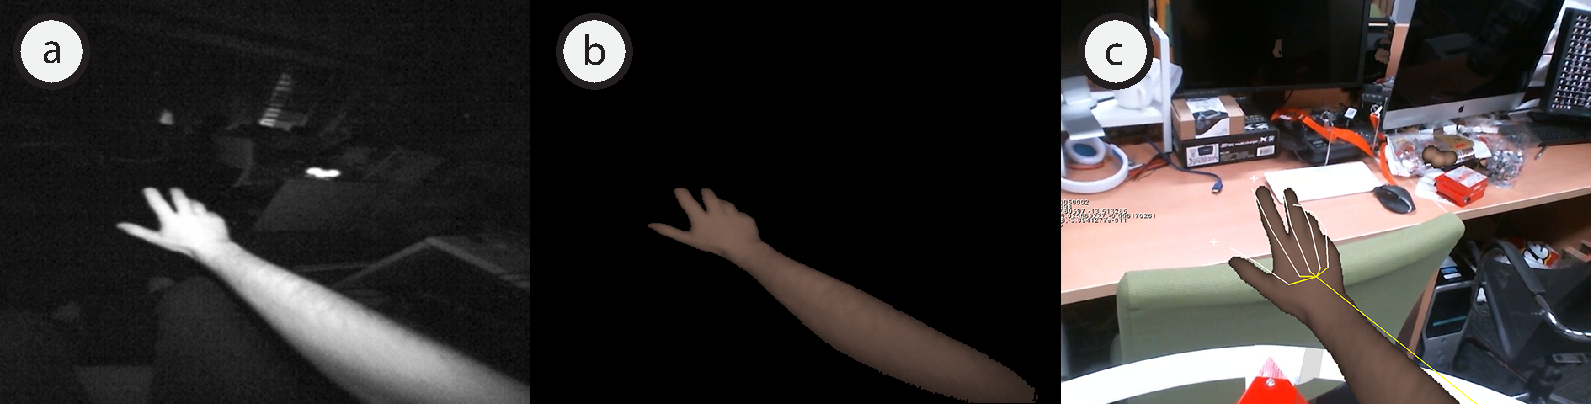
\includegraphics[width=1\linewidth]{figures/eval/ET/HandsVisual.pdf}
  \caption{User's virtual body image segmentation and composition into the physical representation.}
  \label{fig:eval-ET-hands}
\end{figure}

In the user side, the hands are captured using an IR camera mounted on the front of the HMD. The camera provides $110\deg$ field of view which covers HMD FoV, and thus it is possible to capture user hands with no cropped areas. Though the resolution of the cameras are relatively low (640x240), up sampling step is necessary to smooth out the edges. The advantages of using IR camera compared with RGB camera is the possibility to capture objects close to the camera using the returned intensity, in this case, hands and body usually maintains close distance to the HMD, and thus their visuals are captured effectively. However there is a resulting noise from the background. A nonlinear filtering function is applied on the captured images, this function removes the pixels which color intensity are below a certain threshold:

\begin{equation}
\label{eq:hands_correction}
Filter(P)=
\begin{cases}
    P^{\frac{1}{Gamma}}, & \text{if } P^{\frac{1}{Gamma}} \geq threshold \\
    0,                  & \text{otherwise}
\end{cases} 
\end{equation}
\[
 \emph{P}\in\left [ 0,1 \right ] 
\]


\Figure{fig:eval-ET-hands} shows the procedure to extract and segment arms visuals from the background. (a) is the raw data captured by the IR camera, a noticeable amount of background noise is presented in the captured images. (b) shows the process of filtering the noise from the background. A color correction is also used to tint and match the visual appearance of the hands with the human skin color. And finally (c) is the super imposed hands image into the remote visuals after applying perspective correction to match the capture FoV from the cameras with FoV of the HMD. The user would observe the hands being placed correctly within his field of vision corresponding to the actual placement of his body.



\subsection{System Diagram}


The overall data flow and main components of the system are shown in Figure \ref{fig:eval-ET-system}. The robot side follows the design aspects of the toolkit described in \Chapter{ch:impl}. An additional component was added to this system at the representation side, that is a pico-projector mounted on the head of the robot which is used for hands displaying and projection. User hand images are streamed remotely to robot side, and are projected from robot's point of view using a pico projector mounted on its head. Those hands are aligned with user hands position and motion, and allows the remote participants to see the gesture of his hands. \Figure{fig:eval-ET} (B) \& (C)  shows the hands being projected on a trivial surface, in which user hand gesture can be seen remotely. Depending on projector's lumens, the hands might be difficult to see in a well lit room. In current implementation, a 65 lumen projector to render the hands was sufficient in dim lighting condition. 


\begin{figure}[t!]
  \centering
  \captionsetup{justification=centering}
  \includegraphics[width=1\linewidth]{figures/eval/ET/SystemDiagram.pdf}
  \caption{System data flow between user, representation, and the used meta-model.}
  \label{fig:eval-ET-system}
\end{figure}

\subsection{EDD Meta-model}

The meta-model for this type of representation alteration system is shown in \Figure{fig:eval-ET-metamodel}, which reflects the mediating layer in the previously shown diagram \Figure{fig:eval-ET-system}. This model uses two different representation meta-blocks for the virtual body representation: \textbf{Hands Display} block to provide visual feedback of user's hand locally, and \textbf{Hands Projection} block to project the body visuals remotely on the robot side. \textbf{Hands Capture} block handles the visual captures, and produces details about the Hands (hands images provider) that can be used to segment and extract hands information locally and remotely. These information are provided to the robot side for projection, and to the user to be super-imposed locally. The flow of the information is highlighted by the green arrows. Using this meta-model, it is possible to alter the hands display or projection using transfer blocks if needed (changing hands model used, hands attributes such as color and length, and even the number of fingers). 


\begin{figure}[htpb]
  \centering
  \captionsetup{justification=centering}
  \includegraphics[width=1\linewidth]{figures/eval/ET/ET_meta.png}
  \caption{Screen-shot of Enforced Mutual Presence meta-model using EDD editor.}
  \label{fig:eval-ET-metamodel}
\end{figure}


\subsection{Evaluation of Presence}
To evaluate the effectiveness of representation alteration, Enforced Mutual Presence meta-model was used to add virtual hands to the representation, and to provide the user visual feedback of his body visuals being rendered remotely. 

\begin{figure}[b]
  \centering
	  \includegraphics[width=1\linewidth]{figures/eval/ET/EnvironmentSetup.pdf}
  \captionsetup{justification=centering}
  \caption{Representation alteration evaluation room setup: (a) Avatar navigation room, (b) user operation room.}
  \label{fig:eval-setup}
\end{figure}

\textbf{Hypothesis:} The addition of the virtual hands increases the sense of presence for the user, and enhances the engagement of operator in the remote place during the operation. 


\textbf{Experiment Setup:} The experiment was conducted in a living room setup. The room was divided into tow parts. Avatar navigation room was well lit, and contained several objects, tables and chairs as can bee seen in
\Figure{fig:eval-setup}(a). This setup reflects one of the intended applications of this system, the use of such platforms into our daily life environments. Several participants did not have a previous knowledge about the layout of the room. The experiments were conducted individually for each of the participants. The participants were situated in an isolated small room that contained the tools for controlling the robot \Figure{fig:eval-setup}(b). Tracking devices for the head and hands are provided in the HMD. The avatar system is connected over a wireless network with the user side.

\textbf{Participants:} For this study, 10 subjects joined the experiment (8 Males and 2 Females). The age range for the participants is 22 to 32 years (Mean: 26 - SD: 3.6). Basic information were collected from each participant at the beginning of the experiment, 3 out of 10 reported they are unable to see stereoscopic contents using virtual reality devices due to their eyes condition.

\textbf{Procedure:} The experiment was divided into the following cases:
\begin{itemize}
  \item Case 1: Operate the robot without hands presentation (enforced presence meta-model not used).
  \item Case 2: Operate the robot with hands feedback (enforced presence meta-model used).
\end{itemize}



To avoid evaluation bias, the participants were divided into two groups, each group experienced the system in a different case order from the other. Group A experience case 1 followed by case 2, while Group B experience case 2 followed by case 1. During the experiment, we observed user's behavior when the hands were enabled and disabled. A questionnaire was asked after each case to report their subjective experience of the system: interactivity, body presence, involvement level, as well as disturbance or confusion while using it. 


\begin{figure}[t!]
  \centering
	  \includegraphics[width=1\linewidth]{figures/eval/ET/ResultsCombined.pdf}
  \captionsetup{justification=centering}
  \caption{Representation alteration user study for Group A and B, as well as the combined results for both groups.}
  \label{fig:eval-results}
\end{figure}
\begin{table}[h!]
\centerline{
    \begin{tabular}{rrrrr}
    \toprule
    \multicolumn{5}{c}{\textbf{Group A}} \\
    & \multicolumn{2}{c}{No Hands} & \multicolumn{2}{c}{With Hands} \\
    \textbf{Question} &  \textbf{Mean} & \textbf{SD} &  \textbf{Mean} & \textbf{SD}\\
    Natural Interaction  & 4.6 & 1.52 &  5.2   & 0.84 \\
    Body presence  & 4.4 & 1.14 & 5.2   & 0.83 \\
    Involvement level  & 4.8 & 0.84 &  5     & 0.71 \\
    Disturbed or confused  & 3 & 2 &  2.4   & 1.67 \\
    \midrule
    \multicolumn{5}{c}{\textbf{Group B}} \\
    & \multicolumn{2}{c}{No Hands} & \multicolumn{2}{c}{With Hands} \\
    \textbf{Question} &  \textbf{Mean} & \textbf{SD} &  \textbf{Mean} & \textbf{SD} \\
    Natural Interaction & 3.17 & 1.33  &  3.67   & 0.52 \\
    Body presence & 4.17 & 1.33 &  4.4   & 0.52 \\
    Involvement level & 3.5 & 1.38 & 4.8   & 0.75\\
    Disturbed or confused & 4.67 & 1.03 &  2.4   & 1.52\\
    \bottomrule
    \end{tabular}%
}
  \begin{tablenotes}
      \small
      \item Answer Range: 1: Low - 6: High.
    \end{tablenotes}%
  \centering
  \captionsetup{justification=centering}
  \caption{Questionnaire results for Group A and B with and without hands representation. }
  \label{tab:eval-ET-Quest}%
\end{table}


\textbf{Results:} \Figure{fig:eval-results} shows the results after evaluating Group A and Group B, and details of groups answers are listed in \Table{tab:eval-ET-Quest}. It can be noticed that the presentation of virtual hands helps to enhance the state of operation, and reduces the confusion about body presence. The data shows that the lack of hands in both conditions resulted higher deviation in the measured data mainly for level of disturbance and confusion. Group A which experienced the system without hands at the beginning showed a noticeable increment in body presence and natural interaction, and reported their excitement when they saw their hands being ``available''. When the hands was presented, participants were using their hands more actively for pointing, gesturing and communication. For Group B they started using the system with their hands being presented, several participants found it rather trivial for their hands to be there where they expect them to be. In contrast with Group A, when the hands were removed in Group B, they reported less involvement and more confusion about the operation (with hands $2.4\pm1.52$ compared to no hands $4.67\pm1.03$). Some participants expressed their feeling as ``taking away part of their body'' during the experiment. 


From the previous experiment, it can be shown that the body presentation (despite being virtually substituted) helps to increase the overall sense of presence and minimizes the disembodied feeling of lacking some parts of the body (level of confusion). Using representation alteration meta-modeling design, it is possible to overcome such limitations of body presentation.


\subsection{Public Demonstration \& Discussion}

The system has been demonstrated publicly in three major international conferences (SIGGRAPH Asia 2014 Emerging Technologies \cite{saraiji2014enforced}, Augmented Human 2015 \cite{saraiji2015mutual}, and ICAT 2015 \cite{saraiji2015development}) in which attendees experienced several variations of the system (addition of haptic feedback) as shown in \Figure{fig:ET-siggraph}. The core concept was maintained in which the virtual representation of the body was added to augment the perception of presence, and to maintain the sense of body ownership. The benefits of this system were not just the enhancement of bodily presence, but also extended into social and usability situations.



Although the projected hands did not serve to provide any actual physical actions, such as moving, grasping, or manipulating other physical objects, however, they acted as an important social cue. The body visuals transfer has played a role of being a medium to communicate and transfer the fact of a human being in operation, not just a robotic/physical medium that used to capture and transfer information. The ability to use non-verbal communication to infer the need or the state of the user in operation to the remote participants. 

\begin{figure}[t!]
  \centering
  \captionsetup{justification=centering}
  \includegraphics[width=0.9\linewidth]{figures/eval/SIGGRAPH/ET_Siggraph.pdf}
  \par
  \caption{Demonstration of Mutual Enforced Presence system: users interacting through virtual hands with others despite the lack of physical representation of the hands.}
  \vspace*{\floatsep}
  \label{fig:ET-siggraph}
\end{figure}

The other advantage of using such hybrid system in which a non-physical component incorporated into was to overcome the physical constraints. The users found it much easier to express what they needed by just pointing their hands into the objects even in far locations. The projected hands served as a medium that expanded their reachability beyond the physical bounds of their real arms. This shows the advantages of using a mixture of virtual/physical representations to overcome certain constraints and bounds inherited within the human body.

%%%%%%%%%%%%%%%%%%%%%%%%%%%%%%%%%%%%%%%%%%%%%%%%%%%%%%%%%%%%%%%%%%%%%%%%%%%%%%%%%%%%%%%%%%

\pagebreak
\section{HUG Project}
\label{sec:eval-hug}

\begin{comment}
\begin{figure}[htpb]
  \centering
	  \includegraphics[width=1\linewidth]{figures/eval/MetaModels/HUG-Meta.pdf}
  \captionsetup{justification=centering}
  \caption{Use of Meta-Modeling approach to address HUG Project (physical disability).}
  \label{fig:eval-hug-MetaModelReq}
\end{figure}
\end{comment}

Overcoming the physical limitations of human body was one of the goals of human augmentation research. Physical limitations does not have to be just a form of a lost modality, but any physical constraint could be considered as a limitation of the body. \textit{HUG Project} demonstrates a scenario in which EDD meta-modeling was used to resolve a physical disability of a 90-year-old lady. The project has started as a collaboration with Ducklings Japan \cite{ducklingsjp} in late 2015 to design a system which can provide the accessibility for the lady to participate in a remote wedding ceremony of her grandson (the CEO of Ducklings inc.). The project lasted for almost three months (August - October 2015) in which the remote presence system had to be tested and used at the wedding ceremony. The lady was hospitalized with a physical disability of her body that restricted her neck motion significantly. 


\begin{figure}[h!]
  \centering
	  \includegraphics[width=1\linewidth]{figures/eval/HUG/Overview.pdf}
  \captionsetup{justification=centering}
  \caption{HUG Project design requirements overview.}
  \label{fig:usability-hug-overview}
\end{figure}

An overview of the discussed scenario is shown in \Figure{fig:usability-hug-overview}, in which the disabled lady uses a remote representation to access the wedding ceremony. In such situation which a physical disability is presented to the user, if a \textit{Direct body transfer} meta-model was used then the same modality disability will be reflected in the representation. To address this, \textit{Topology reconfiguration} meta-model is used to change the postural topology of the body schema. For this particular scenario, \Figure{fig:concept-EDD-HUG} shows the target meta-model of this system in which the eye gaze is used to substitute head rotation (disabled modality) of the representation. Other modalities can also be used, however, the eye gaze was a suitable input for the head rotation to minimize the number of tracking devices attached to the lady.


\begin{figure}[t!]
  \centering
  \includegraphics[width=0.95\linewidth]{figures/eval/EDD/EDD-HUG.pdf}
  \captionsetup{justification=centering}
  \caption{An overview of the target meta-model for modality substitution in HUG Project.}
  \label{fig:concept-EDD-HUG}
\end{figure}

\subsection{Meta-model Design}

Initial tests were conducted using the toolkit discussed previously in \Chapter{ch:impl}, however, it was not sufficient to be used in a social event such as the wedding ceremony. Thus an alternative avatar system was required. To resolve this, Softbank Pepper robot was used as ``body host'' which just mediates the postural schema of the grandmother (hands, heads motion), and a custom stereoscopic camera module was developed and embedded into the robot to provide the visual sensory mapping. Both postural and sensory modalities were integrated into the EDD framework to be used for interaction modeling. 

Since the lady was not capable to use her head motion to operate the robot, an alternative operation modality was required to use instead of her physical head motion, or else the representation will also inherit the same physical limitation of the user. To resolve this, the eye gaze is used as an input modality to the system and was mapped into the head rotation of the representation. Thus the lady had full capability to rotate the head of the robot using two axes: 
\begin{itemize}
    \item Tilt axis: mapped with the vertical motion of eye pupil.
    \item Yaw axis:  mapped with the horizontal motion of eye pupil.
\end{itemize}

\begin{figure}[t!]
  \centering
	  \includegraphics[width=1\linewidth]{figures/eval/HUG/Meta.pdf}
  \captionsetup{justification=centering}
  \caption{A screen-shot of HUG Projection meta-model using topology reconfiguration.}
  \label{fig:usability-hug-meta}
\end{figure}


\begin{figure}[b!]
  \centering
	  \includegraphics[width=1\linewidth]{figures/eval/HUG/Hug.pdf}
  \captionsetup{justification=centering}
  \caption{HUG Project: eyegaze substituting head motion.}
  \label{fig:usability-hug}
\end{figure}

FOVE HMD was used to capture the eye gaze movement converted into normalized 2D coordinates, and to provide her the visual feedback from the wedding. The eye gaze modality is decoupled into horizontal and vertical motion, which are mapped into rotation angles using Tilt and Yaw filter blocks. These filters acts as non-linear functions which are defined for each axis separately, and used to remap the motion of the eyes [-1,+1] into rotational values in degrees [-90,+90]. The chosen function (designed as set of key points) sustains the rotation within limited range of eye gaze motion, and provides non-linearity mapping along the edge to start rotating the head. The results of the angles conversion function are coupled to a rotation block (as Euler angles) and mapped to a joint which would correspond to the head joint of the robot. The overall EDD meta-model used with the transfer blocks to achieve topology reconfiguration is shown in \Figure{fig:usability-hug-meta}. This EDD model acts as a high level design tool that can be easily manipulated and alternated to remodel the control mechanism and body structure. 
 

The final results of this model were sufficient to produce sense of agency toward the robot although the control mechanism does not match how our body moves. This result was concluded based on the feedback received by the lady in which she expressed her feeling of being physically in the ceremony and her active involvement when interacting with the remote attendees \Figure{fig:usability-hug}. 


\subsection{Discussion}

This scenario had showcases that the concept of operation alteration could benefit wide spectrum of physically impaired people to gain back the sense of the lost modality by re-configuring their body schema. 

Several reasons could have contributed in her immerse with the system and biased her experience to be as ``believable'' sense of presence despite being aware that she was using mediated tools and she was not physically there in her own body. Psychological factors such as the emotional attachment toward the groom played an important factor to build up the social context of the experience. The second factor is the use of an immersive display (HMD) for the first time affected her sensory and perceptual experience of involvement. The sensory matching of her visual feedback (stereo vision camera module), and the correlated control of the robot head via through her eye motion created a closed loop system in which she can drive, and gain feedback. This loop created a strong sense of agency toward the artificial body. Lastly, the social context in which the remote participants at the wedding ceremony expressed affection toward her avatar system. The use of human factors in the designing the experience creates mutual social involvement in which the observers can understand that the person within the shell of the robot is actually a human, which is expressed by body shape and canny motion. 

Topology reconfiguration design approach would result losing the function of the source modality which is used as for the substitution.Although this argument is sound, it is not true all the time. Since in most of the time we do not use our entire body muscles for operation. For example, when seated, our legs usually at rest all the time. The decision of the body configuration is totally driven by the embodied designer which can be the user himself, thus the user can reconfigure his body schema depending on the scenario and state of his body (like body reprogramming/rewiring). This approach is effective in a sense that the users can adapt to the new representation by deploying an existing modality they are accustomed to. The plasticity of our body helps in temporarily reconfiguring our postural mapping and control of the new schema.

%%%%%%%%%%%%%%%%%%%%%%%%%%%%%%%%%%%%%%%%%%%%%%%%%%%%%%%%%%%%%%%%%%%%%%%%%%%%%%%%%%%%%%%%%%

%\pagebreak
\section{Layered Presence}
\label{sec:eval-layeredpresence}

\begin{comment}

\begin{figure}[htpb]
  \centering
	  \includegraphics[width=1\linewidth]{figures/eval/MetaModels/LP-Meta.pdf}
  \captionsetup{justification=centering}
  \caption{Use of MetaModeling approach to address Layered Presence (body limitations).}
  \label{fig:eval-LP-MetaModelReq}
\end{figure}

\end{comment}

\begin{figure}[htpb]
  \centering
  \includegraphics[width=0.7\linewidth]{figures/eval/Layered/Teaser.png}
\captionsetup{justification=centering}
\caption{Layered Presence: combining visual feedback from two different locations. }
\label{fig:eval-layered-overview}
\end{figure}


Our bodies are inherently limited to operate or perceive to/from a single point of interaction. For example we see from a single location which our body is presented at, similarly our actions follows the same physical constraints. The use of Telepresence and Telexistence robots for example expands our spatial awareness, however the same limitations are also presented in such type of systems. To challenge such body limitation, Layered Presence provides an approach to expand our modalities function and from one-to-one mapping to one-to-many mapping. 

The proposed system addresses the previous mapping point by using multiple Telexistence robots (based on the embodiment toolkit) that are synchronized with user’s motion, and provides real-time visual and auditory feedback to the user. Robots are represented as layers of perception (originally discussed in \Section{sec:concept-ModAlt}), in which the information represented by each layer can be visual, auditory, or haptic feedback. These layers are blended based on the saliency found in them, and presented to the user’s feedback displays. User’s eye gaze is used as the main interaction modality for layers information presentation. Eye gaze is tracked and used to identify the target layer to be highlighted among the other layers based on the saliency information dominance. The layer user is looking at becomes focused while the other layers are defocused using an artificial depth of field effect, that maintains the optical flow in the peripheral vision of the user. Figure \ref{fig:eval-layered-overview} shows the proposed system in action in which the user perceives two different locations simultaneously. This system is addressed using EDD meta-modeling as illustrated in \Figure{fig:eval-EDD-LP}. The meta-model reflects the idea of modality expansion by mapping body's modalities into multiple representations. Layered Perception transfer block is responsible to combine/expand the modalities inputs/outputs between the user and representations. Details about the design and implementation of this transfer block are described in the following sections.

\begin{figure}[h!]
  \centering
  \includegraphics[width=0.95\linewidth]{figures/eval/EDD/EDD-LP.pdf}
  \captionsetup{justification=centering}
  \caption{An overview of the target meta-model for addressing one-to-many body mapping situations.}
  \label{fig:eval-EDD-LP}
\end{figure}

\subsection{Design overview}


To realize the idea of overcoming the limited body perceptual awareness, a Layered Presence system has been developed using EDD framework. The system uses Telexistence robots (based on the embodiment toolkit) that are synchronized with user’s motion, and provides real-time visual and auditory feedback to the user. \Figure{fig:eval-layered-system} shows an overview of Layered Presence data flow from multiple representations. This interaction uses the eye gaze as an input to the system to determine which spot the user is looking at, and based on this input, the system controls the focus of the layers to the corresponding layer user is looking at. To determine the candidate layer that should be in focus, visual saliency maps are generated for each layer that contains the ``interesting'' information from the corresponding representations. Such blending mechanism provides seamless visual feedback of the multiple layers, and maintains the awareness of multiple locations. 

\begin{figure}[h!]
  \centering
  \includegraphics[width=0.7\linewidth]{figures/eval/Layered/SystemFlow.png}
\captionsetup{justification=centering}
\caption{Layered Presence: perception flow from multiple avatars.}
\label{fig:eval-layered-system} 
\end{figure}

\subsection{Saliency Map Generation}
Saliency maps in this method are responsible to represent the presence of remote participants as a weight map generated for each captured frame while taking to consideration the temporal factor of the frames. The process of generating the saliency maps is done by a combination of two image analysis and features extraction methods. First the layers are processed for human presence, the procedure is done by applying Haar cascades classifier on each captured frame and the results are rectangles set representing the detected faces regions. These rectangles are expanded proportionally to their size to cover user body size (manually tuned, Width factor: 200\%, Height factor: 400\%). In practice however, using facial detection only fails to provide continuous tracking of presented people for several reasons such as partial occlusion of the face, lighting conditions, and resolution of the captured images. Also relying on facial detection only limits the visual saliency maps to capture the information of moving objects in scene. We addressed this limitation by adding a second layer of tracking using optical flow detection in the layers. Lucas-Kanade method was used to track scene features points for changing. When local changes occur in the layers, motion vectors are recorded for later registration in the corresponding saliency map of the layer. \Figure{fig:LP-saliency} (A) shows the detected motion vectors.


\begin{figure}[t!]
  \centering
  \captionsetup{justification=centering}
  \includegraphics[width=1\linewidth]{figures/eval/Layered/weights.png}
  \caption{Saliency maps generation for the layers.}
  \label{fig:LP-saliency}
\end{figure}

Next, the saliency maps are filled with weight of 1 for the pixels corresponding to the registered feature points and facial regions for each layer. To avoid the presence of hard edges along the detected regions, a Gaussian blur filter is applied to the saliency maps. To assist feature tracking consistency over time, a temporal process is applied to the calculated maps, a window of 500ms of previously calculated frames is used to calculate the weighted sum of the final saliency map. Using this procedure, the saliency maps maintained higher consistency in both tracking and representation of participant’s area in video frames. \Figure{fig:LP-saliency} (B) shows the final saliency map for a single layer. 

\subsection{Layer Fusing}
Fusing the layers, or mixing them, is considered the final step of this method to deliver the layers to the user view area. One of the main considerations in LP is the user should maintain clear visuals and auditory feedback from the location he is engaged at, while being aware of the other locations simultaneously. Firstly, the layers are fused together based on the weight of each layer which is assigned based on user's eye gaze. Each layer's weight is calculated by sampling saliency map corresponding to each layer using eye gaze coordinates. 


\begin{figure}[htpb]
  \centering
  \captionsetup{justification=centering}
  \includegraphics[width=1\linewidth]{figures/eval/Layered/fusing.png}
  \caption{Two different locations fused together with an artificial depth of field.}
  \label{fig:LP-fusing}
\end{figure}

In preliminary experiments of layer fusing, we used a basic alpha blending to all layers based on the calculated weight of each layer, however we found that its difficult for the users to clearly distinguish the visuals of the layers due to visual overlapping between all locations. To address this issue, we considered using a similar phenomenon seen in image reflection over window glass. Basically this phenomenon of reflection and transparency of window glass allows to see two different locations simultaneously as well as the ability to focus at different depths that would result blurriness of objects in the background of both locations (depth of field). Using this phenomenon, a pseudo model was defined that defines a focal value for each layer, that is basically driven from the calculated layer weight, is used to control the amount of shallowness of layers out of focus. \Figure{fig:LP-fusing} shows the final results of fusing two layers using the proposed method.

\subsection{Layered Presence Meta-modeling}

The meta-model for layered presence is shown in \Figure{fig:eval-LP-metamodel}. The model reflects the main components interacting with the user, the robot, and the intermediate transfer blocks. Two new transfer blocks encapsulates the functionality layering the visuals and auditory feedback:
\begin{itemize}
\item \textbf{Layered vision block}: receives several visual sources (can be determined by the designer) from the representations side. Calculates the saliency information based on the eye gaze of the user. The eye gaze modality block can be changed to a different modality type as long as it can provide a compatible output (Vec2). This block calculates the fused layers, and stores the results as vision data type, which can be linked to the user block.

\item \textbf{Layered Audio block}: provides the functionality to layer the audio feedback from multiple sources based on the calculated layers weights from the [Layered Vision] block. The output of this block is audio type which can be directed to the user block.
\end{itemize}


\begin{figure}[t!]
  \centering
  \captionsetup{justification=centering}
  \includegraphics[width=1\linewidth]{figures/eval/Layered/LayeredMetaModel.png}
  \caption{A screen-shot of layered presence meta-model using EDD editor.}
  \label{fig:eval-LP-metamodel}
\end{figure}

\subsection{Applications}

\begin{figure}[b!]
  \centering
  \captionsetup{justification=centering}
  \includegraphics[width=1\linewidth]{figures/eval/Layered/Applications.pdf}
  \par
  \caption{Layered presence applications. (A) interacting with remote location while being in VR environment, (B) use of video see-through while teleconferencing, and (C) layering media contents.}
  \vspace*{\floatsep}
  \label{fig:LP-applications}
\end{figure}

This method can be expanded to more than just Telexistence related applications. By using the concept of layered perception, its possible to generalize the layers to be media or even interactive applications, and apply the same procedure in combining them into a single space. Also, we define two modes of viewpoint (Egocentric \& Exocentric), in which are based on user's point of view and how the user perceives the remote environment or the layers.
\newline
\textbf{Egocentric Applications:} The user in this type of application is immersed with the task he is doing, for example when the user is being engaged in a virtual reality game while wearing HMD. By using the concept of LP, the game it self is also considered as a layer that can be fused with other layers with eye gaze enabled. By using this method, the user is capable to be simultaneously engaged with the activity he is doing as well as with remote discussion. \Figure{fig:LP-applications} (A) shows an example of LP with virtual game. Also by using a video see-through HMD, its possible to consider the local location as a layer, and thus it can be seamlessly fused with a remote location as shown in \Figure{fig:LP-applications} (B). 
\newline
\textbf{Exocentric Applications:} In this category of applications, the user perceives the layers from an external display with an external eye tracker mounted into the display. The contents of the display (application, visual media, etc.) can thus be considered as a layer of presence, while remote robots are blended with contents of the display. \Figure{fig:LP-applications} (C) shows an example of interacting with a software while being engaged in a simultaneous meeting in two different locations. 


\subsection{Public Demonstration \& Discussion}

\begin{figure}[b!]
  \centering
  \captionsetup{justification=centering}
  \includegraphics[width=1\linewidth]{figures/eval/SIGGRAPH/LP_SIGGRAPH.pdf}
  \par
  \caption{Demonstration of Layered Presence at SIGGRAPH 2016 Anahiem. User connected to three different locations in parallel.}
  \vspace*{\floatsep}
  \label{fig:LP-siggraph}
\end{figure}

After demonstrating Layered Presence system in SIGGRAPH 2016 \cite{saraiji2016layered}, several observations and highlights were collected out of the attendees who experienced it. The demonstration consisted of three layers: 
\begin{itemize}
\item Local layer A: provided a video see-through into the local space which the user is located at. The user can observe his body through it and his local surroundings.
\item Remote layer B: located at a spatially different location from where the user is located at, in the demonstration it was referred to be in Japan (by setting a background image of Japanese site).
\item Remote layer C: similarly to layer B, this layer was referred to be in Paris. 
\end{itemize}

At each layer, a person was located which enabled direct communication with the user of the system. \Figure{fig:LP-siggraph} shows an overall layout of the experience setup used in which the participants experienced simultaneous multiple location perceptual presence. The low latency, consistent motion and optical flow that was maintained across the three layers provided seamless experience of spatial consistency. The corresponding representations (Layer B,C) were following the exact motion of the user head, which enabled mutual communication with remote participants. The usage of eye-gaze as an input to layer selection helped as an intuitive trigger to the region of interest. Most of the participants reported as being ``co-located'' with three persons, where in fact they were only facing one person. They even tried to reach by their hand to the remote participants during conversation to confirm whether they were actually located beside them or not. The fact of using such validation method shows the effectiveness of Layered Presence to convince the visual/kinesthetic modalities that the three layers coexist spatially together. When they failed to ``touch'' the remote participants, they reported as their body being a ``phantom'', not physically existed any more. This transitional state between physical and phantom body highlights the role of the body to validate the spatial localization, and can be viewed as an indicator to the effectiveness of perception layering. That is the user is aware his local space as well as the remote locations, and trying to interact in between them.



%%%%%%%%%%%%%%%%%%%%%%%%%%%%%%%%%%%%%%%%%%%%%%%%%%%%%%%%%%%%%%%%%%%%%%%%%%%%%%%%%%%%%%%%%%


\pagebreak
\section{MetaLimbs}
\label{sec:eval-metalimbs}
\begin{comment}

\begin{figure}[htpb]
  \centering
	  \includegraphics[width=1\linewidth]{figures/eval/MetaModels/ML-Meta.pdf}
  \captionsetup{justification=centering}
  \caption{Use of MetaModeling approach to address Meta Limbs (physical disability or body limitation).}
  \label{fig:eval-ML-MetaModelReq}
\end{figure}
\end{comment}


\begin{figure}[h!]
  \centering
	  \includegraphics[width=1\linewidth]{figures/eval/MetaLimbs/MetaLimbs_Adaptation.jpg}
  \captionsetup{justification=centering}
  \caption{MetaLimbs: use of body topology reconfiguration to alter limbs mapping.}
  \label{fig:eval-metalimbs-overview}
\end{figure}

The last use-case discussed in this chapter is MetaLimbs \Figure{fig:eval-metalimbs-overview}. MetaLimbs addresses the ability to change body schema and postural topology in a way we can alter our limbs functions and model. We developed a proof of concept system that expands the number of limbs to four independently operated arms. Previous work discussed the topic of using an artificial prosthesis to augment or support body locally \cite{stelarc1980thirdhand,parietti2014bracing} required a long period of time to adapt to the newly added arms in order to perform tasks, or was partially operated using an autonomous system which thus disembodies the newly added arms. In this work, we discuss the possibility of remapping our body to achieve immediate adaptation and operation for the new limbs, and to maintain the sense of embodiment towards these additional limbs. 

As discussed in \Section{sec:concept-OpAlt}, Topology reconfiguration meta-model is used to change the body schema topology by reassigning existing modalities to new ones in the representation. The goal is to maintain the sense of embodiment and ownership towards the additional limbs by mapping its functionality to existing joints of the body, thus when the joint moves, the artificial limb moves in accordance to its motion. For MetaLimbs, the topology reconfiguration meta-model maps legs motion to the newly added arms as viewed in \Figure{fig:eval-EDD-ML}. The arms also provide force feedback to the legs so the user can be aware of objects touching the hands (creating closed-loop feedback system). Further details about this system are described in the following sections.

\begin{figure}[t!]
  \centering
  \includegraphics[width=0.95\linewidth]{figures/eval/EDD/EDD-Meta.pdf}
  \captionsetup{justification=centering}
  \caption{An overview of the target meta-model for remapping body limbs.}
  \label{fig:eval-EDD-ML}
\end{figure}

\subsection{Design Overview}

MetaLimbs uses two 7 degrees of freedom anthropomorphic robotic arms that can be mounted on the user back. These arms can function as an extension of the human body, and function as extra limbs, thus expanding the number of arms into four arms. The main consideration in designing such a system is control mechanism of the new limbs in which it can provide independent motion of the four arms, and driven by the user to maintain the sense of ownership toward the new limbs. Existing work in Supernumerary Robotic Limbs (SRL) \cite{parietti2016supernumerary} uses a supportive approach for the additional limbs, which are mainly used as assistant limbs instead of being embodied with user's actions. For MetaLimbs, the approach used here is user-driven, that is to use existing body modalities to alter the operation of the new limbs. The approach used here is to use leg/feet motion to drive the arms, thus limb mapping model is used. \Figure{fig:eval-metalimbs-system} shows an overview of body configuration in which feet motion are retargeted into the hand's motion.


\begin{figure}[t!]
  \centering
	  \includegraphics[width=1\linewidth]{figures/eval/MetaLimbs/MetaLimbsOverview.pdf}
  \captionsetup{justification=centering}
  \caption{Re-configuring body schema mapping using feet motion.}
  \label{fig:eval-metalimbs-system}
\end{figure}


\subsection{Meta-model Design}


In EDD modeling categories, Topology Reconfiguration meta-model addresses this type of interactions by redirecting an existing body modality output to a different part. For MetaLimbs, this can be achieved by redirecting legs motion into the artificial arms motion.


\begin{figure}[t!]
  \centering
	  \includegraphics[width=1\linewidth]{figures/eval/MetaLimbs/MetaLimbs_EDD.png}
  \captionsetup{justification=centering}
  \caption{A screen-shot of MetaLimbs meta-model using EDD editor.}
  \label{fig:eval-metalimbs-EDD}
\end{figure}

To realize this model, \Figure{fig:eval-metalimbs-EDD} shows the meta-model for MetaLimbs system. Tracking markers were used to capture the spatial position and orientation of user's legs. One marker per feet, and single marker as a reference for the waist. \textbf{Arm IK} transfer block was used to reconstruct the arm posture based on the feet posture by calculating the inverse kinematics model of the arms. The resulting posture is provided to a body block which is directed into the robotic representation of the arms. The representation block handles the joints values (vector of angular data for each link) to drive the robotic arms. All calculations are done in real-time to match the intended actions of the user.

One of the advantages of using meta-modeling is the ability to apply non-linear mapping to the motion. For example, for high-precision control of the arms, the spatial resolution of the control can be scaled down so large motions are mapped to smaller motion trajectories. These types of control derivations can be easily done on a meta-level design.



\subsection{Public Demonstration \& Discussion}

MetaLimbs system has been showcased in SIGGRAPH 2017 Emerging Technologies, in which more than 200 attendees experience the system for the first time. Generally speaking, the users were capable to adapt to the new body structure within the first 3 minutes of operation, in which they were able to hand shake, hold objects, and interact with their own arms \Figure{fig:ET-siggraph}. The main drawback in the operation was the mechanical latency of driving the arms. The participants spent the initial time to understand the speed limits and the spatial reachability of the arms (about 2 mins on average). Some participants were capable to develop fast adaptation to the new body schema and to interact using their own physical arms and the new limbs by doing coordinating actions. Usually, this type of motor-skill learning requires several trial and error until getting sufficient operation of the limbs.

\begin{figure}[t!]
  \centering
  \captionsetup{justification=centering}
  \includegraphics[width=0.85\linewidth]{figures/eval/SIGGRAPH/ML_SIGGRAPH.pdf}
  \par
  \caption{MetaLimbs at SIGGRAPH 2017 Los Angeles. Users adapted to the artificial arms are able to interact using them as being part of their body.}
  \vspace*{\floatsep}
  \label{fig:ET-siggraph}
\end{figure}

This mechanism of body restructuring and schema adaptation would open the possibilities for new types of human augmentation functions to use on-body robotics extensions to facilitate a variety of tasks. Also, it can be used as an approach for prosthetic limbs control which can provide an immediate alteration and substitution of the missing limb.

One of the limitations this system lacks is the proprioceptive feedback regarding the posture of the arms. Currently, the arms are being driven one way by the legs move, and the user can understand their spatial position based on the legs posture (open loop system). However, when the arms are adjusted by an external factor (like handshaking, or blocked by an object), the user will need to have visual feedback to maintain an understanding of the posture of the arms. Our biological arms, on the other hand, we are aware of their posture at any moment thanks to proprioceptive feedback, the inner structure and spatial position of each joint. To address this issue, we are considering to investigate in using EMS\footnote{Electrical muscle stimulation, the use of electrical impulses to cause muscle contraction.} feedback to create a closed-loop system, thus arms' posture would affect legs' posture. 




%\updatedtext{
\section{Summary \& Reflections}
%Effect of going beyond one own physical space into spatially different one (build on Telexistence)
%Idea of changing own body and how it reflects the new abilities we were unborn with
%Idea of expanding the perceptual capabilities beyond our limited physical range
% Tx Vehicle
% Enforce Presence
% HUG Project
% Layered Presence
% MetaLimbs

This chapter has demonstrated five use-cases and scenarios in which EDD meta-modeling approach helped addressing body limitations and physical disabilities and provided the tools to modulate the body schema and representation mapping. Also, it described how the use of such meta-level modeling approaches helps to alter the perception of space and physical limits while maintaining the embodied sense of ownership and agency during the operation.  Concepts related to expanding the body physical limits and constraints using hybrid virtual and physical forms, exploring the topic of ubiquitous presence and expanded spatial perception, and reforming the topology of the human body structure by adding extra limbs and mapping them to existing modalities were discussed. 


%\section{Reflections}

General observations of users who experienced the previously discussed projects have shared in common the active involvement through the newly provided embodied abilities and functions. In some projects, this effect was more dominant than others (Enforced Mutual Presence, Layered Presence, and MetaLimbs) in which users experienced new body function that was not presented before into their disposal (extended arms,  expanded spatial awareness, and multiple arms respectively). In the scenarios which the body schema or representation has been altered from the original body form and interaction, users spent varied amount of time to learn and adapt to the new representation. The adaptation to the new body schema reflected the level of plasticity our bodies and cognitive abilities can achieve. When changing the body mapping, our understanding of the new body would also change as well as the way we embody our actions through it. For example, Enforced Mutual Presence showed that adding hands representation would significantly change our body awareness and level of presence. Similarly for MetaLimbs, when our body mapping was altered that the legs functions as arms, our cognitive understanding of body topology is changed accordingly. This alteration assisted to create new image of our new limbs affordabilities and what it can do, thus the users of the system quickly learned to use and maneuver through the new body schema.

One of the important means that EDD provides when addressing a body augmentation design problem is the flexibility to change the design and mapping of the body transfer model. Thus, the same system can be used by different users using different interactions and body mapping while, depending on the design, the embodied interaction is maintained. For example, for HUG Project scenario, it is possible to reuse the same system for a user with different physical impairment by changing body mapping and substituting the disability. Such flexibility is inherited from the meta-modeling approach used in the design of the system.

%Enforced Mutual Presence has highlighted the role of body to support and raise the feeling of presence and awareness of being. It showed that the body, when non-tangible actions are sufficient, can be substituted into a different form, which once the user's adapted to 



%}


